\section{Flip-Flop D \label{sec:s3}}

\begin{center}
	\begin{minipage}{12cm}
		\begin{tcolorbox}[title=Actividad 3]
			 Un flip-flop D puede construirse a partir de dos latch tipo D en cascada (configuración MASTER-SLAVE) de acuerdo al siguiente diagrama:\enter
			 
			 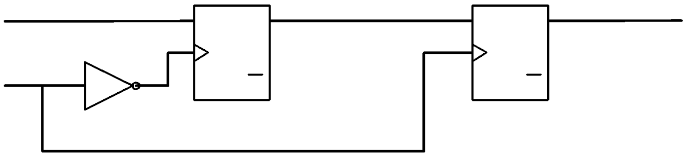
\includegraphics[scale=0.3,center]{FlipFlopD.png}
			 Usar dos instancias del latch D del inciso 2. Repetir los pasos del inciso 1.
		\end{tcolorbox}	
	\end{minipage}
\end{center}

La visualización RTL, del flip-flop D implementado con la directiva \textit{(keep)}, se muestra en la \autoref{fig:FlipFlop_D_Keep_RTL} y sin esta directiva en la \autoref{fig:FlipFlop_D_NoKeep_RTL}. Se observa que dentro de estas instancias se tiene la descripción por flujo de datos de bajo nivel, o sea, la conexión entre compuertas lógicas (Ver \autoref{fig:FlipFlop_D_Keep_RTL2} y \autoref{fig:FlipFlop_D_NoKeep_RTL2}). Los módulos se diferencian en que el circuito con \textit{keep} conserva más compuertas lógicas que el que no usa la directiva, además de mantener intactas a las señales internas.

La visualización con el \textit{Technology Map Viewer}, del flip-flop D implementado con la directiva \textit{keep}, se muestra en la \autoref{fig:FlipFlop_D_Keep_TMV} y sin esta directiva en la \autoref{fig:FlipFlop_D_NoKeep_TMV}. En la \autoref{fig:FlipFlop_D_Keep_TMV2} y \autoref{fig:FlipFlop_D_NoKeep_TMV2}, se observa que dentro de las instancias se generan celdas lógicas. Los módulos se diferencian en que el circuito con \textit{keep} implementa una celda lógica por cada señal interna declarada en la instancia, mientras que el circuito sin \textit{keep} emplea una sola celda lógica para todo el circuito instanciado. Nótese que, la señal que conecta un latch D con el otro, también genera una celda lógica para el circuito con \textit{keep}, ya que es una señal interna del módulo.

Las simulaciones sin retardos se visualizan en la \autoref{fig:FlipFlop_D_Keep_Wave} para el flip-flop D con directiva \textit{keep} y en la \autoref{fig:FlipFlop_D_NoKeep_Wave} para el flip-flop D sin directiva. Ambos circuitos funcionan de la misma manera, de tal forma que 

\begin{itemize}
	\item \textbf{Si D = 0}: La salida adquiere un valor bajo.
	\item \textbf{Si D = 1}: La salida adquiere un valor alto.
\end{itemize}

Nótese que los cambios en la salida ocurren unicamente cuando CLK tiene un flanco de subida.

Las simulaciones con retardos (modo lento a 85°C) se visualizan en la \autoref{fig:FlipFlop_D_Keep_Wave85} para el flip-flop D con directiva \textit{keep} y en la \autoref{fig:FlipFlop_D_NoKeep_Wave85} para el flip-flop D sin directiva. Se observa que, debido a que se simuló en el peor de los escenarios, la señal de salida Q, tarda en actualizar su valor en ambas simulaciones, no obstante, para el caso del circuito con \textit{keep}, el retardo es ligeramente mayor en comparación con el circuito sin \textit{keep}.

En los Anexos se localiza la descripción del flip-flop D. Tomando como instancia al latch D, declarado en la actividad 2, se realizó la descripción del módulo de forma estructural.

\begin{figure}[ht]
	\centering
	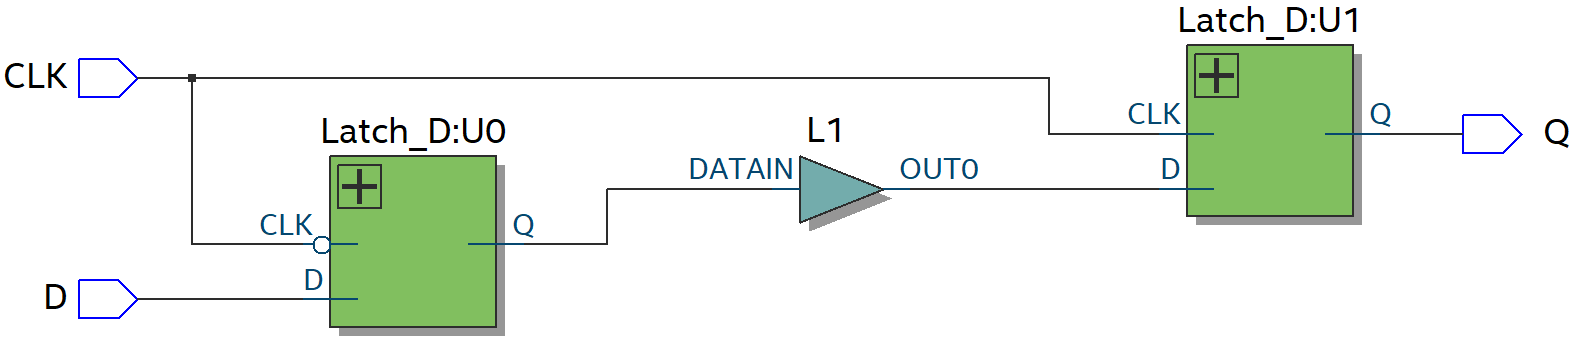
\includegraphics[scale=0.39]{FlipFlop_D_Keep_RTL.png}
	\caption{Diagrama RTL del flip-flop D, descrito con la directiva \textit{keep}. \label{fig:FlipFlop_D_Keep_RTL}}
\end{figure}

\begin{figure}[ht]
	\centering
	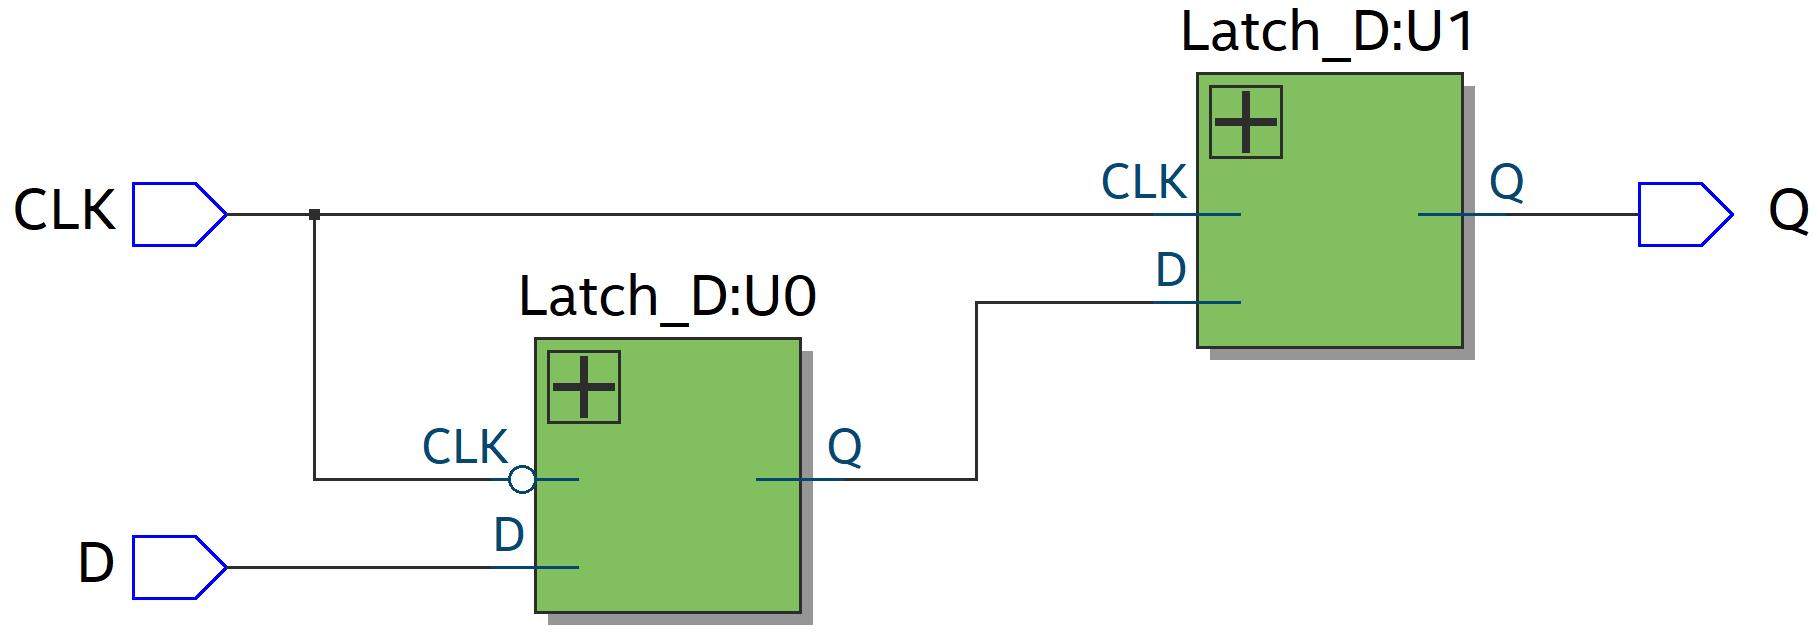
\includegraphics[scale=0.34]{FlipFlop_D_NoKeep_RTL.png}
	\caption{Diagrama RTL del flip-flop D, descrito sin la directiva \textit{keep}. \label{fig:FlipFlop_D_NoKeep_RTL}}
\end{figure}

\begin{figure}[ht]
	\centering
	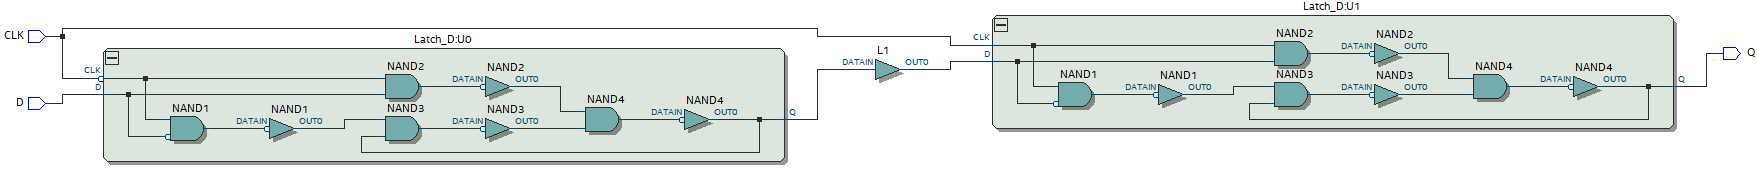
\includegraphics[scale=0.36]{FlipFlop_D_Keep_RTL2.png}
	\caption{Diagrama RTL del flip-flop D, descrito con la directiva \textit{keep} (acercamiento al interior de la instancia). \label{fig:FlipFlop_D_Keep_RTL2}}
\end{figure}

\begin{figure}[ht]
	\centering
	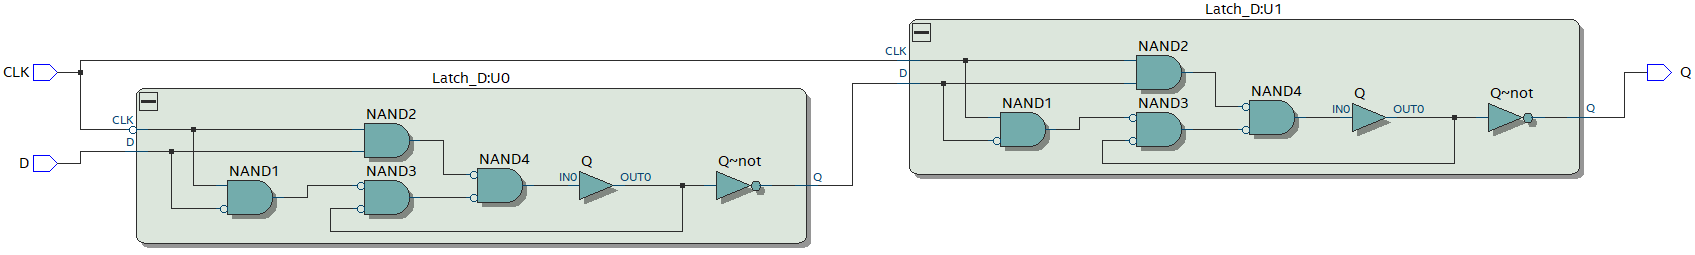
\includegraphics[scale=0.37]{FlipFlop_D_NoKeep_RTL2.png}
	\caption{Diagrama RTL del flip-flop D, descrito sin la directiva \textit{keep} (acercamiento al interior de la instancia). \label{fig:FlipFlop_D_NoKeep_RTL2}}
\end{figure}

\begin{figure}[ht]
	\centering
	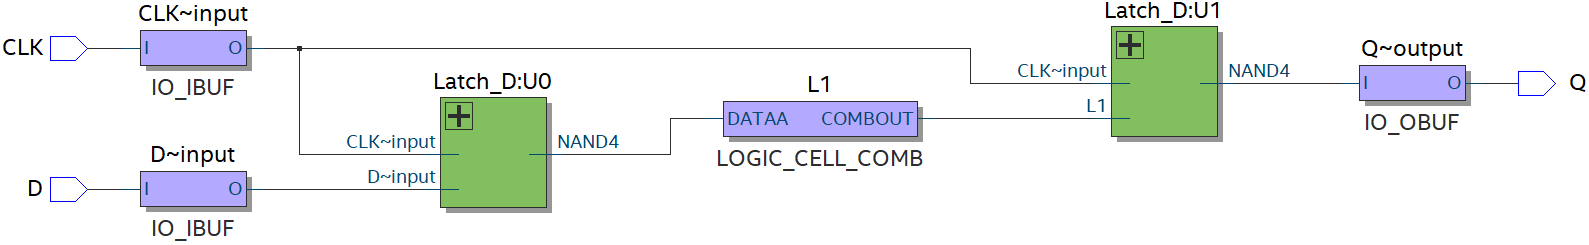
\includegraphics[scale=0.38]{FlipFlop_D_Keep_TMV.png}
	\caption{Flip-Flop D (descrito sin la directiva \textit{keep}) visto desde el \textit{Technology Map Viewer}. \label{fig:FlipFlop_D_Keep_TMV}}
\end{figure}

\begin{figure}[ht]
	\centering
	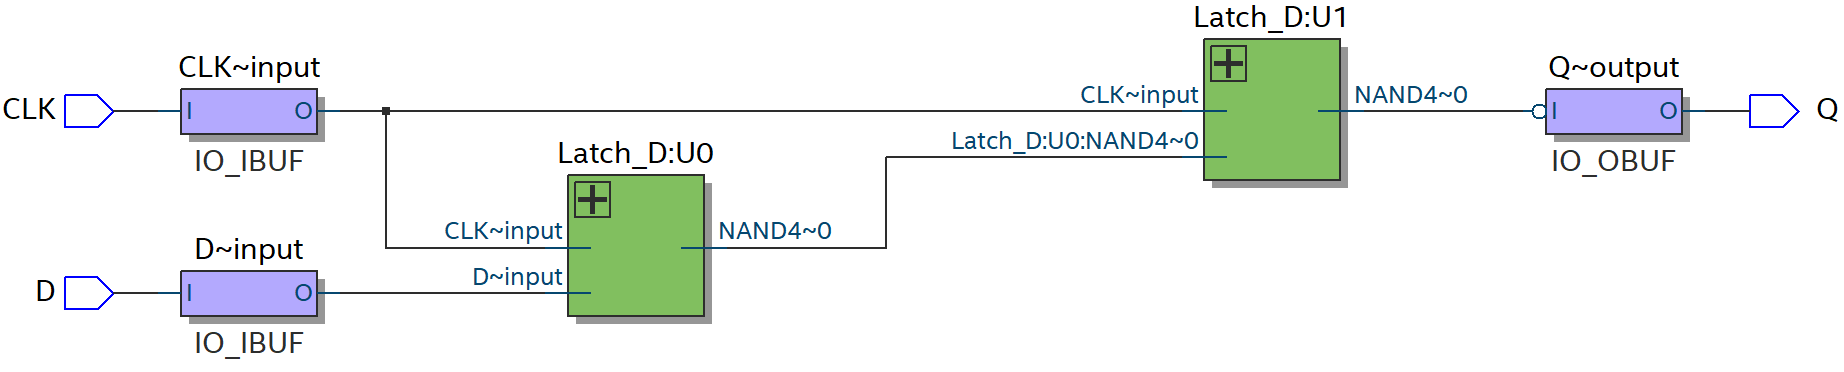
\includegraphics[scale=0.33]{FlipFlop_D_NoKeep_TMV.png}
	\caption{Flip-Flop D (descrito sin la directiva \textit{keep}) visto desde el \textit{Technology Map Viewer}. \label{fig:FlipFlop_D_NoKeep_TMV}}
\end{figure}

\begin{figure}[ht]
	\centering
	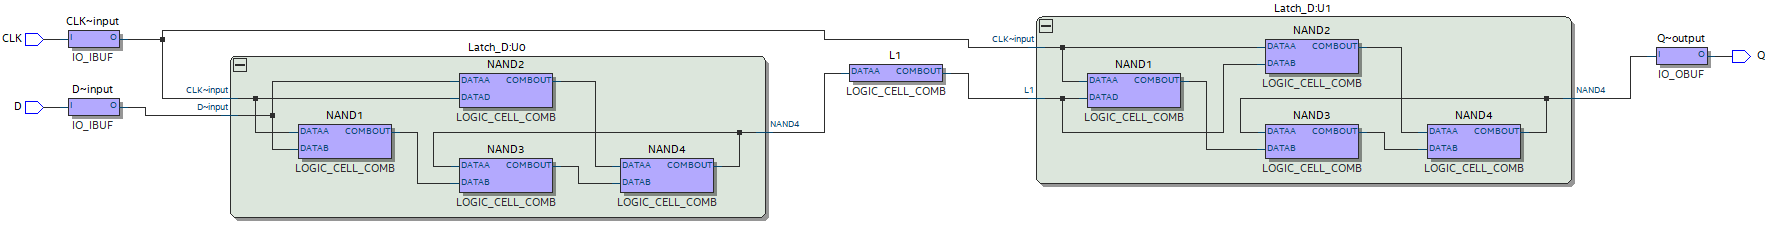
\includegraphics[scale=0.36]{FlipFlop_D_Keep_TMV2.png}
	\caption{Flip-Flop D (descrito sin la directiva \textit{keep}) visto desde el \textit{Technology Map Viewer} (acercamiento al interior de la instancia). \label{fig:FlipFlop_D_Keep_TMV2}}
\end{figure}

\begin{figure}[ht]
	\centering
	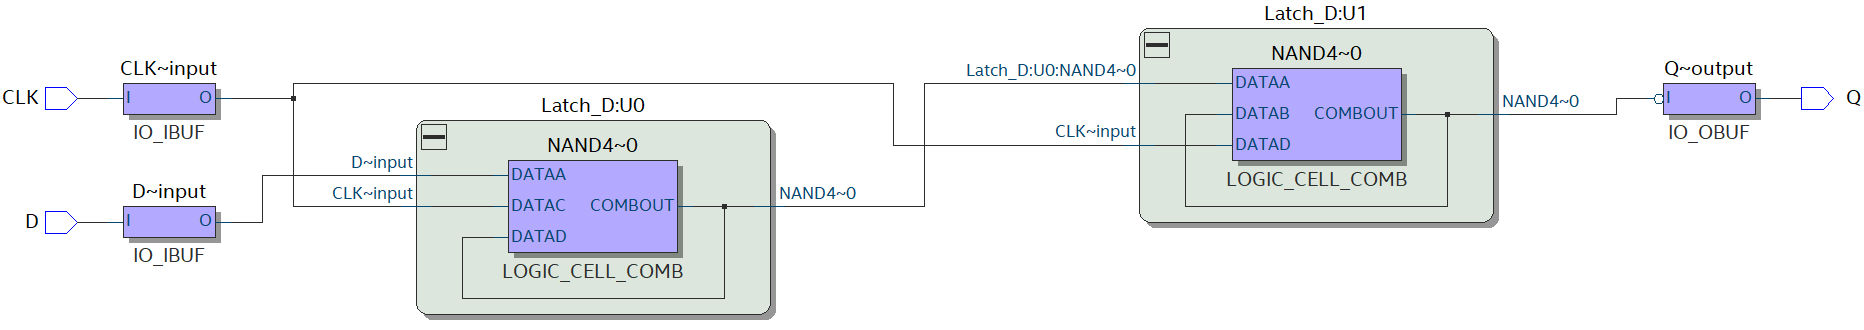
\includegraphics[scale=0.33]{FlipFlop_D_NoKeep_TMV2.png}
	\caption{Flip-Flop D (descrito sin la directiva \textit{keep}) visto desde el \textit{Technology Map Viewer} (acercamiento al interior de la instancia). \label{fig:FlipFlop_D_NoKeep_TMV2}}
\end{figure}

\begin{figure}[ht]
	\centering
	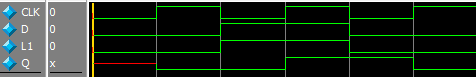
\includegraphics[scale=1.3]{FlipFlop_D_Keep_Wave.png}
	\caption{Simulación sin retardos del flip-flop D (descrito con la directiva \textit{keep}) en el visor de formas de onda de ModelSim. \label{fig:FlipFlop_D_Keep_Wave}}
\end{figure}

\begin{figure}[ht]
	\centering
	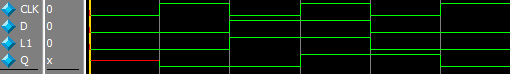
\includegraphics[scale=1.2]{FlipFlop_D_NoKeep_Wave.png}
	\caption{Simulación sin retardos del flip-flop D (descrito sin la directiva \textit{keep}) en el visor de formas de onda de ModelSim. \label{fig:FlipFlop_D_NoKeep_Wave}}
\end{figure}

\begin{figure}[ht]
	\centering
	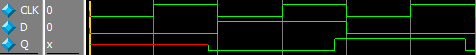
\includegraphics[scale=1.3]{FlipFlop_D_Keep_Wave85.png}
	\caption{Simulación con retardos del flip-flop D (descrito con la directiva \textit{keep}) en el visor de formas de onda de ModelSim. \label{fig:FlipFlop_D_Keep_Wave85}}
\end{figure}

\begin{figure}[ht]
	\centering
	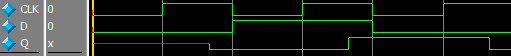
\includegraphics[scale=1.2]{FlipFlop_D_NoKeep_Wave85.png}
	\caption{Simulación sin retardos del flip-flop D (descrito sin la directiva \textit{keep}) en el visor de formas de onda de ModelSim. \label{fig:FlipFlop_D_NoKeep_Wave85}}
\end{figure}